\chapter{Proof}
\label{sec:proof}


\section{Consistency}

As described in Chapter~\ref{sec:description}, a snapshot would be
inconsistent if it captured an event, but not an earlier event that
caused it. To provide an intuitive example, let $A$ be some event that
caused another event, $B$.  For example, $A$ could be a new user added
to a database. Event $B$ could be a change to another user's friend
list to include $A$. If we captured $B$ in our snapshot, but not $A$,
our snapshot would contain the friend relation, but not the new
user. See Figure~\ref{fig:consistency} for examples of consistent and
inconsistent snapshots.

More formally, here is the statement that we want to prove: {\em let
  $A$ and $B$ be events in our system, where $B$ was caused by
  $A$. Our goal is to prove that if $B$ was captured in our snapshot,
  then $A$ must have been as well.}

Figure~\ref{fig:consistentoverlap} demonstrates the concept that we're
going to prove here.

\begin{figure}[!htbp]
  \centering
  \caption{This is all possible event orders given that A caused B. Yellow and green boxes are node freeze windows and the dotted blue line is the overlap where the snapshot is taken. We can see that A is captured by the snapshot if B is, meaning that the snapshot is consistent.} 
  \label{fig:consistentoverlap}
  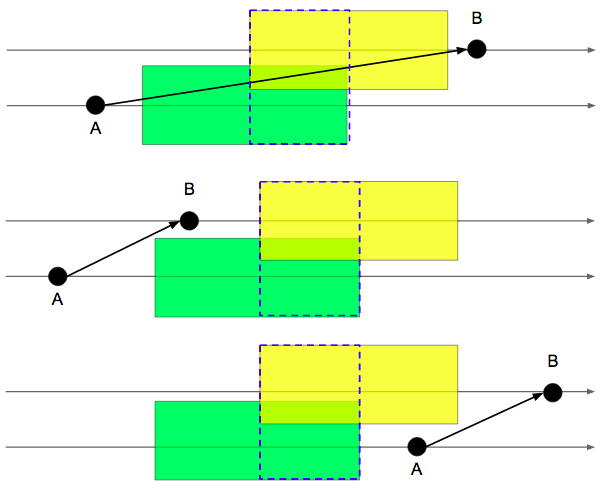
\includegraphics[width=0.75\textwidth]{consistentoverlap.png}
\end{figure}

First, define $T_A$ to be the (objective) time at which $A$ occurred
and $T_B$ to be the (objective) time at which $B$ occurred. Since $A$
caused $B$, we know that $A$ must have taken place before $B$, meaning
$T_A < T_B$.

In Chapter~\ref{sec:approach}, we shows that CASTS guarantees
that all of the freeze windows of the nodes in our system will overlap
when we are taking a snapshot. In other words at some point in time or
for some time period, all nodes will be frozen.  During this interval,
the cluster as a whole will not confirm completion of to write
events. Therefore, when we are considering the order of events, we can
collapse that whole interval into a single event $F$ and we can
consider the start time of the interval to be the time of the event
$T_F$.

Assume, for the sake of contradiction, that there is a series of
events that could violate the invariant that an event would only be
captured in a snapshot if all events that caused that event were
captured as well. More specifically, let us have events $C$ and $D$
such that $C$ caused $D$. Assume that it is possible for $D$ to have
been captured in the snapshot while $C$ was not.

Recall from Chapter~\ref{sec:approach} that each node's portion of the
snapshot occurs when that node first freezes. No other events will
occur on that node between when it takes its snapshot (i.e., the
beginning of its freeze interval) and $F$, the moment when all nodes
are frozen. By our assumption above, if $D$ was included in the
snapshot, it must have happened before $F$, meaning $T_D <T_F$. Since
$C$ caused $D$, it must have happened temporally before $D$.  Since
$C$ was not captured in the snapshot, it must have happened either
after $F$, or between its node's freeze start time and $F$. The first
is clearly a contradiction, since $D$ happened before $F$. The second
is a contradiction, because then $C$ would not have completed before
$F$, so it could not have caused anything before $F$. So, we know that
our original assumption that $D$ was captured and $C$ was not must
have been incorrect and, therefore, our statement must be true for any
pair of events in the cluster that are causally related. To extend
this further, since our statement is true for any two events in our
system with a causal relationship, we know that our snapshot must be
consistent.

\section{Performance}

There are several performance characteristics that need to be
considered to preserve Ceph's performance while implementing CASTS. 
First, we need to consider the impact of
delaying writes for a freeze. Since each node freezes for twice the
uncertainty bounds that is determined by the time protocol, the
magnitude of the uncertainty bounds is dependent on which time
synchronization protocol is used. In Chapter \ref{sec:results}, we
analyze the uncertainty that NTP provides and discuss what impact CASTS
would have on a Ceph cluster if NTP is used as the
time synchronization protocol. However, as long as a time
synchronization protocol could provide uncertainties in the 10-20
millisecond range, yielding 20-40 millisecond
freeze %% TODO this is inaccurate but idk what we want to do about it
windows, CASTS should not impact the cluster's performance in
a way noticeable to client applications.  Also, freeze windows of each
of the nodes are offset from each other as they freeze for their own
individual uncertainty bounds, which means that the point in time
where the whole Ceph cluster is frozen is much shorter.

In this section, we consider the impact on network link quality of
CASTS. We need to be assured that CASTS does not
require significant amounts of bandwidth which would cause network
congestion within a Ceph cluster. Since most Ceph clusters are already
running a time synchronization protocol like NTP, CASTS does
not require any extra messages during the synchronization phase. The
freeze phase also does not require any extra messages. The number of
success/failure messages required in the confirmation phase is $O(n)$
in the size of the cluster and thus would not have an excessive impact
on the performance of the cluster (because each message would be only
a few bytes). In the replication phase, the remote cluster needs to
read the data from the local one, but this cost is inherent to any
snapshotting algorithm.

Finally, we need to consider whether CASTS will place a
significant computational burden on nodes. Each primary node needs to
send its data to the remote cluster. This should not impact the
performance of the primaries, since it should only take a small amount
of time to send all its data provided data is sent in differences
between snapshots rather than complete sets. Even if it did take some
time to send the data, read and write requests could still be
addressed by prioritizing those requests above the requests for the
objects from the remote cluster. Sending all of the data out at once
could require nontrivial bandwidth, but since it is distributed
throughout the Ceph cluster, the choke point would be the bandwidth
from the local cluster to the remote cluster, which should be large
and not a concern if we prioritize normal client traffic over the
inter-cluster traffic.

Based on our analysis, CASTS should not degrade the
performance of a Ceph cluster.
